\documentclass[nooutcomes]{ximera}
%\documentclass[space,handout,nooutcomes]{ximera}

\usepackage{epsfig}

\graphicspath{
  {./}
  {figures/}
  {../laode}
  {../laode/figures}
}

\usepackage{epstopdf}
\epstopdfsetup{outdir=./}

\usepackage{morewrites}
\makeatletter
\newcommand\subfile[1]{%
\renewcommand{\input}[1]{}%
\begingroup\skip@preamble\otherinput{#1}\endgroup\par\vspace{\topsep}
\let\input\otherinput}
\makeatother

\newcommand{\EXER}{}
\newcommand{\includeexercises}{\EXER\directlua{dofile(kpse.find_file("exercises","lua"))}}

\newenvironment{computerExercise}{\begin{exercise}}{\end{exercise}}

%\newcounter{ccounter}
%\setcounter{ccounter}{1}
%\newcommand{\Chapter}[1]{\setcounter{chapter}{\arabic{ccounter}}\chapter{#1}\addtocounter{ccounter}{1}}

%\newcommand{\section}[1]{\section{#1}\setcounter{thm}{0}\setcounter{equation}{0}}

%\renewcommand{\theequation}{\arabic{chapter}.\arabic{section}.\arabic{equation}}
%\renewcommand{\thefigure}{\arabic{chapter}.\arabic{figure}}
%\renewcommand{\thetable}{\arabic{chapter}.\arabic{table}}

%\newcommand{\Sec}[2]{\section{#1}\markright{\arabic{ccounter}.\arabic{section}.#2}\setcounter{equation}{0}\setcounter{thm}{0}\setcounter{figure}{0}}
  
\newcommand{\Sec}[2]{\section{#1}}

\setcounter{secnumdepth}{2}
%\setcounter{secnumdepth}{1} 

%\newcounter{THM}
%\renewcommand{\theTHM}{\arabic{chapter}.\arabic{section}}

\newcommand{\trademark}{{R\!\!\!\!\!\bigcirc}}
%\newtheorem{exercise}{}

\newcommand{\dfield}{{\sf dfield9}}
\newcommand{\pplane}{{\sf pplane9}}
\newcommand{\PPLANE}{{\sf PPLANE9}}

% BADBAD: \newcommand{\Bbb}{\bf}

\newcommand{\R}{\mbox{$\Bbb{R}$}}
\newcommand{\C}{\mbox{$\Bbb{C}$}}
\newcommand{\Z}{\mbox{$\Bbb{Z}$}}
\newcommand{\N}{\mbox{$\Bbb{N}$}}
\newcommand{\D}{\mbox{{\bf D}}}
\usepackage{amssymb}
%\newcommand{\qed}{\hfill\mbox{\raggedright$\square$} \vspace{1ex}}
%\newcommand{\proof}{\noindent {\bf Proof:} \hspace{0.1in}}

\newcommand{\setmin}{\;\mbox{--}\;}
\newcommand{\Matlab}{{M\small{AT\-LAB}} }
\newcommand{\Matlabp}{{M\small{AT\-LAB}}}
\newcommand{\computer}{\Matlab Instructions}
\newcommand{\half}{\mbox{$\frac{1}{2}$}}
\newcommand{\compose}{\raisebox{.15ex}{\mbox{{\scriptsize$\circ$}}}}
\newcommand{\AND}{\quad\mbox{and}\quad}
\newcommand{\vect}[2]{\left(\begin{array}{c} #1_1 \\ \vdots \\
 #1_{#2}\end{array}\right)}
\newcommand{\mattwo}[4]{\left(\begin{array}{rr} #1 & #2\\ #3
&#4\end{array}\right)}
\newcommand{\mattwoc}[4]{\left(\begin{array}{cc} #1 & #2\\ #3
&#4\end{array}\right)}
\newcommand{\vectwo}[2]{\left(\begin{array}{r} #1 \\ #2\end{array}\right)}
\newcommand{\vectwoc}[2]{\left(\begin{array}{c} #1 \\ #2\end{array}\right)}

\newcommand{\ignore}[1]{}


\newcommand{\inv}{^{-1}}
\newcommand{\CC}{{\cal C}}
\newcommand{\CCone}{\CC^1}
\newcommand{\Span}{{\rm span}}
\newcommand{\rank}{{\rm rank}}
\newcommand{\trace}{{\rm tr}}
\newcommand{\RE}{{\rm Re}}
\newcommand{\IM}{{\rm Im}}
\newcommand{\nulls}{{\rm null\;space}}

\newcommand{\dps}{\displaystyle}
\newcommand{\arraystart}{\renewcommand{\arraystretch}{1.8}}
\newcommand{\arrayfinish}{\renewcommand{\arraystretch}{1.2}}
\newcommand{\Start}[1]{\vspace{0.08in}\noindent {\bf Section~\ref{#1}}}
\newcommand{\exer}[1]{\noindent {\bf \ref{#1}}}
\newcommand{\ans}{\textbf{Answer:} }
\newcommand{\matthree}[9]{\left(\begin{array}{rrr} #1 & #2 & #3 \\ #4 & #5 & #6
\\ #7 & #8 & #9\end{array}\right)}
\newcommand{\cvectwo}[2]{\left(\begin{array}{c} #1 \\ #2\end{array}\right)}
\newcommand{\cmatthree}[9]{\left(\begin{array}{ccc} #1 & #2 & #3 \\ #4 & #5 &
#6 \\ #7 & #8 & #9\end{array}\right)}
\newcommand{\vecthree}[3]{\left(\begin{array}{r} #1 \\ #2 \\
#3\end{array}\right)}
\newcommand{\cvecthree}[3]{\left(\begin{array}{c} #1 \\ #2 \\
#3\end{array}\right)}
\newcommand{\cmattwo}[4]{\left(\begin{array}{cc} #1 & #2\\ #3
&#4\end{array}\right)}

\newcommand{\Matrix}[1]{\ensuremath{\left(\begin{array}{rrrrrrrrrrrrrrrrrr} #1 \end{array}\right)}}

\newcommand{\Matrixc}[1]{\ensuremath{\left(\begin{array}{cccccccccccc} #1 \end{array}\right)}}



\renewcommand{\labelenumi}{\theenumi}
\newenvironment{enumeratea}%
{\begingroup
 \renewcommand{\theenumi}{\alph{enumi}}
 \renewcommand{\labelenumi}{(\theenumi)}
 \begin{enumerate}}
 {\end{enumerate}\endgroup}

\newcounter{help}
\renewcommand{\thehelp}{\thesection.\arabic{equation}}

%\newenvironment{equation*}%
%{\renewcommand\endequation{\eqno (\theequation)* $$}%
%   \begin{equation}}%
%   {\end{equation}\renewcommand\endequation{\eqno \@eqnnum
%$$\global\@ignoretrue}}

%\input{psfig.tex}

\author{Martin Golubitsky and Michael Dellnitz}

%\newenvironment{matlabEquation}%
%{\renewcommand\endequation{\eqno (\theequation*) $$}%
%   \begin{equation}}%
%   {\end{equation}\renewcommand\endequation{\eqno \@eqnnum
% $$\global\@ignoretrue}}

\newcommand{\soln}{\textbf{Solution:} }
\newcommand{\exercap}[1]{\centerline{Figure~\ref{#1}}}
\newcommand{\exercaptwo}[1]{\centerline{Figure~\ref{#1}a\hspace{2.1in}
Figure~\ref{#1}b}}
\newcommand{\exercapthree}[1]{\centerline{Figure~\ref{#1}a\hspace{1.2in}
Figure~\ref{#1}b\hspace{1.2in}Figure~\ref{#1}c}}
\newcommand{\para}{\hspace{0.4in}}

\usepackage{ifluatex}
\ifluatex
\ifcsname displaysolutions\endcsname%
\else
\renewenvironment{solution}{\suppress}{\endsuppress}
\fi
\else
\renewenvironment{solution}{}{}
\fi

%\ifxake
%\newenvironment{matlabEquation}{\begin{equation}}{\end{equation}}
%\else
\newenvironment{matlabEquation}%
{\let\oldtheequation\theequation\renewcommand{\theequation}{\oldtheequation*}\begin{equation}}%
  {\end{equation}\let\theequation\oldtheequation}
%\fi

\makeatother



\title{Quadrilaterals}
\author{Brad Findell}
\begin{document}
\begin{abstract}
Proof. 
\end{abstract}
\maketitle


\begin{problem}
Adapted from Ohio's 2017 Geometry released item 13. 

Two pairs of parallel lines intersect to form a parallelogram as shown.  
\begin{image}
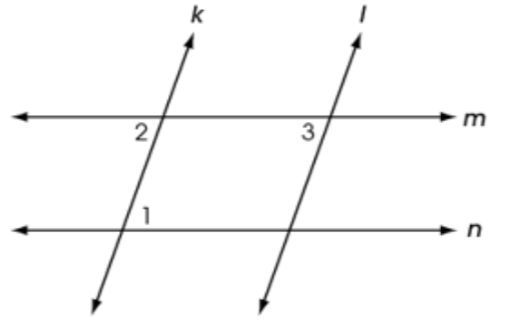
\includegraphics{Q13.png}
\end{image}
Complete the following proof that opposite angles of a parallelogram are congruent: 

\begin{enumerate}
\item $\angle 1 \cong \angle 2$ as \wordChoice{\choice{opposite angles}\choice[correct]{alternate interior angles}\choice{corresponding angles}}
for parallel lines \wordChoice{\choice[correct]{$m$ and $n$}\choice{$k$ and $l$}}.
\item $\angle 3 \cong \angle 2$ as \wordChoice{\choice{opposite angles}\choice{alternate interior angles}\choice[correct]{corresponding angles}}for parallel lines \wordChoice{\choice{$m$ and $n$}\choice[correct]{$k$ and $l$}}.
\item Then $\angle 1 \cong \angle 3$ because they are both congruent 
to $\angle 2$. 
\end{enumerate}
\end{problem}

\begin{problem}
Adapted from Ohio's 2018 Geometry released item 21. 

Given the parallelogram $WXYZ$, prove that $\overline{WX}\cong\overline{YZ}$. 

\begin{image}
\definecolor{qqqqff}{rgb}{0.,0.,1.}
\begin{tikzpicture}[line width=0.8pt,line cap=round,line join=round,x=1.0cm,y=1.0cm] % ,>=triangle 45
\clip(-0.5,-0.6) rectangle (5.5,2.5);
\draw (0.,0.)-- (4.,0.);
\draw (4.,0.)-- (5.,2.);
\draw (5.,2.)-- (1.,2.);
\draw (1.,2.)-- (0.,0.);
\draw (1.,2.)-- (4.,0.);
\begin{scriptsize}
\draw [fill=qqqqff] (0.,0.) circle (1.2pt);
\draw[color=qqqqff] (-0.28,-0.03) node {$Z$};
\draw [fill=qqqqff] (1.,2.) circle (1.2pt);
\draw[color=qqqqff] (0.86,2.29) node {$W$};
\draw [fill=qqqqff] (4.,0.) circle (1.2pt);
\draw[color=qqqqff] (4.22,0.07) node {$Y$};
\draw [fill=qqqqff] (5.,2.) circle (1.2pt);
\draw[color=qqqqff] (5.14,2.29) node {$X$};
\end{scriptsize}
\end{tikzpicture}
\end{image}

\fixnote{It really would help to have an online environment that allows students to mark diagrams.}

Complete the proof below: 
\begin{enumerate}
\item $\angle ZWY \cong \angle XYW$ as \wordChoice{\choice[correct]{alternate interior angles}\choice{corresponding angles}\choice{opposite angles}} for parallel segments \wordChoice{\choice[correct]{$\overline{WZ}$ and $\overline{XY}$}\choice{$\overline{WX}$ and $\overline{YZ}$}}.
\item $\angle ZYW \cong \angle XWY$ for the same reason, this time for parallel segments \wordChoice{\choice{$\overline{WZ}$ and $\overline{XY}$}\choice[correct]{$\overline{WX}$ and $\overline{YZ}$}}.
\item $\overline{WY}\cong\overline{YW}$ because a segment is congruent to itself. 
\item $\triangle WYZ \cong \triangle YWX$ by \wordChoice{\choice{SAS}\choice[correct]{ASA}\choice{SSS}}.  
\item Then $\overline{YZ}\cong\overline{WX}$ as corresponding parts of congruent triangles. 
\end{enumerate}
\fixnote{Maybe number the angles.}

\end{problem}


\begin{problem}
Use symmetry to prove properties of parallelograms. 
\begin{image}
% Parallel markings have been commented out
%
\definecolor{uuuuuu}{rgb}{0.267,0.267,0.267}
\definecolor{qqqqff}{rgb}{0.,0.,1.}
\begin{tikzpicture}[line width=0.8pt,line cap=round,line join=round,>=triangle 45,x=1.0cm,y=1.0cm]
\clip(-0.4,-0.45) rectangle (5.4,2.45);
\draw (0.,0.)-- (1.,2.);
%\draw (0.5939,1.1878) -- (0.6677,1.0335);
%\draw (0.5939,1.1878) -- (0.4262,1.1542);
%\draw (0.5,1.) -- (0.5738,0.8457);
%\draw (0.5,1.) -- (0.3323,0.9665);
\draw (1.,2.)-- (5.,2.);
%\draw (3.105,2.) -- (3.,1.865);
%\draw (3.105,2.) -- (3.,2.135);
\draw (5.,2.)-- (4.,0.);
%\draw (4.4061,0.8122) -- (4.332,0.9665);
%\draw (4.4061,0.8122) -- (4.5738,0.8457);
%\draw (4.5,1.) -- (4.4262,1.1543);
%\draw (4.5,1.) -- (4.6677,1.0335);
\draw (4.,0.)-- (0.,0.);
%\draw (1.895,0.) -- (2.,0.135);
%\draw (1.895,0.) -- (2.,-0.135);
\draw (0.,0.)-- (5.,2.);
%\begin{scriptsize}
\draw [fill=qqqqff] (0.,0.) circle (1.2pt);
\draw[color=qqqqff] (-0.16,-0.2) node {$A$};
\draw [fill=qqqqff] (4.,0.) circle (1.2pt);
\draw[color=qqqqff] (4.1,-0.2) node {$B$};
\draw [fill=qqqqff] (1.,2.) circle (1.2pt);
\draw[color=qqqqff] (1.14,2.29) node {$D$};
\draw [fill=qqqqff] (5.,2.) circle (1.2pt);
\draw[color=qqqqff] (5.14,2.29) node {$C$};
\draw [fill=qqqqff] (2.5,1.) circle (1.2pt);
\draw[color=qqqqff] (2.6,1.3) node {$M$};
%\end{scriptsize}
\end{tikzpicture}
\end{image}

Consider a $180^\circ$ rotation about $M$, the midpoint of diagonal $\overline{AC}$.  Show that this rotation maps the parallelogram onto itself.  
\fixnote{The following proof is quite elegant, but some of the details are subtle, especially distinguishing between mapping the sides (i.e., segments) and the lines containing the sides.  Can any of this be omitted or abbreviated?  Which parts might students supply?}
\begin{enumerate}
\item The rotation maps $A$ to $C$ and $C$ to $A$ because a $180^\circ$ rotation about a point on a line takes the line to itself and preserves lengths.
%\item Now a $180^\circ$ rotation about $M$ takes lines not containing $M$ to parallel lines.  
\item The rotation maps $\overleftrightarrow{AB}$ to a parallel line through $C$ (the image of $A$), which by the uniqueness of parallels must 
be $\overleftrightarrow{CD}$.  Similarly, the rotation maps 
$\overleftrightarrow{CD}$ to $\overleftrightarrow{AB}$, 
$\overleftrightarrow{AD}$ to $\overleftrightarrow{CB}$, and
$\overleftrightarrow{CB}$ to $\overleftrightarrow{AD}$.
\item Furthermore, the intersection of $\overleftrightarrow{AB}$ and $\overleftrightarrow{CB}$, which is $B$, must map to the intersection of their images, $\overleftrightarrow{CD}$ and $\overleftrightarrow{AD}$, and that intersection is $D$.  And likewise, $D$ must map to $B$.
\item Because vertices are mapped to vertices, sides are mapped to opposite sides, angles are mapped to opposite angles, and thus the parallelogram is mapped onto itself.  
\end{enumerate}

Now this symmetry proves the following properties \emph{for free}:  

\begin{itemize}
\item opposite sides are congruent (sides are mapped to opposite sides), 
\item opposite angles are congruent (angles are mapped to opposite angles), and 
\item the diagonals bisect each other.

\detail{The $180^\circ$ rotation about $M$ swaps $\overrightarrow{MB}$ 
and $\overrightarrow{MD}$, so they must be opposite rays, and thus $B$, $M$, and $D$ are collinear. \\ Because the rotation preserves lengths, $MB=MD$, so that $M$ is also the midpoint of $\overline{BD}$, which means that the diagonals bisect each other.}
\end{itemize}

\end{problem}


\begin{problem}

Quadrilateral $ABCD$ is a kite as marked.  Prove that $\overleftrightarrow{BD}$ is the perpendicular bisector of $\overline{AC}$. 

\begin{image}
\definecolor{qqqqff}{rgb}{0.,0.,1.}
\begin{tikzpicture}[line cap=round,line width=0.8pt,line join=round,>=triangle 45,x=1.0cm,y=1.0cm]
\clip(-5,-6) rectangle (5,4);
\draw (-3.,0.)-- (0.,-5.);
\draw (-1.440,-2.424) -- (-1.595,-2.516);
\draw (-1.405,-2.484) -- (-1.559,-2.576);
\draw (0.,-5.)-- (3.,0.);
\draw (1.405,-2.484) -- (1.559,-2.576);
\draw (1.440,-2.424) -- (1.595,-2.516);
\draw (3.,0.)-- (0.,2.);
\draw (1.450,0.925) -- (1.550,1.075);
\draw (0.,2.)-- (-3.,0.);
\draw (-1.450,0.925) -- (-1.550,1.075);
\draw (0.,2.)-- (0.,-5.);
\draw (-3.,0.)-- (3.,0.);
\draw (0.,2.)-- (3.,0.);
%\begin{scriptsize}
\draw [fill=qqqqff] (-3.,0.) circle (1.2pt);
\draw[color=qqqqff] (-3.24,0.31) node {$A$};
\draw [fill=qqqqff] (3.,0.) circle (1.2pt);
\draw[color=qqqqff] (3.22,0.21) node {$C$};
\draw [fill=qqqqff] (0.,2.) circle (1.2pt);
\draw[color=qqqqff] (0.14,2.29) node {$B$};
\draw [fill=qqqqff] (0.,-5.) circle (1.2pt);
\draw[color=qqqqff] (-0.26,-5.09) node {$D$};
\draw [fill=qqqqff] (0.,0) circle (1.2pt);
\draw[color=qqqqff] (-0.26,-.26) node {$X$};
%\end{scriptsize}
\end{tikzpicture}
\end{image}

Key theorem:  The points on a perpendicular bisector are exactly those that are equidistant from the endpoints of a segment.  

Proof:  Because $B$ and $\answer[format=string]{D}$ are each $\answer[format=string]{equidistant}$ from $A$ and $\answer[format=string]{C}$, they each must lie on the perpendicular bisector of segment $\answer[format=string]{AC}$, which implies that 
$\overleftrightarrow{BD}$ is its perpendicular bisector.  

\end{problem}

\begin{problem}
Quadrilateral $ABCD$ is a kite as marked.  Prove that $\overleftrightarrow{BD}$ is the perpendicular bisector of $\overline{AC}$. 

\begin{image}
\definecolor{qqqqff}{rgb}{0.,0.,1.}
\begin{tikzpicture}[line cap=round,line width=0.8pt,line join=round,>=triangle 45,x=1.0cm,y=1.0cm]
\clip(-5,-6) rectangle (5,4);
\draw (-3.,0.)-- (0.,-5.);
\draw (-1.440,-2.424) -- (-1.595,-2.516);
\draw (-1.405,-2.484) -- (-1.559,-2.576);
\draw (0.,-5.)-- (3.,0.);
\draw (1.405,-2.484) -- (1.559,-2.576);
\draw (1.440,-2.424) -- (1.595,-2.516);
\draw (3.,0.)-- (0.,2.);
\draw (1.450,0.925) -- (1.550,1.075);
\draw (0.,2.)-- (-3.,0.);
\draw (-1.450,0.925) -- (-1.550,1.075);
\draw (0.,2.)-- (0.,-5.);
\draw (-3.,0.)-- (3.,0.);
\draw (0.,2.)-- (3.,0.);
%\begin{scriptsize}
\draw [fill=qqqqff] (-3.,0.) circle (1.2pt);
\draw[color=qqqqff] (-3.24,0.31) node {$A$};
\draw [fill=qqqqff] (3.,0.) circle (1.2pt);
\draw[color=qqqqff] (3.22,0.21) node {$C$};
\draw [fill=qqqqff] (0.,2.) circle (1.2pt);
\draw[color=qqqqff] (0.14,2.29) node {$B$};
\draw [fill=qqqqff] (0.,-5.) circle (1.2pt);
\draw[color=qqqqff] (-0.26,-5.09) node {$D$};
\draw [fill=qqqqff] (0.,0) circle (1.2pt);
\draw[color=qqqqff] (-0.26,-.26) node {$X$};
%\end{scriptsize}
\end{tikzpicture}
\end{image}

A proof that makes use of triangle congruence:

\begin{image}
\tikzstyle{block} = [rectangle, draw, fill=blue!20, 
    text width=8em, text centered, rounded corners, minimum height=2em]
\tikzstyle{Block} = [rectangle, draw, fill=green!20, 
    text width=10em, text centered, rounded corners, minimum height=3em]
\tikzstyle{implies} = [draw, -latex']

\begin{tikzpicture}[node distance = 1.5cm, auto]
    % Place nodes
    \node [Block] (a) {$\triangle BAD \cong \triangle BCD$};
    \node [block, left of=a, node distance = 4cm] (init) {$AD=CD$};
    \node [block, right of=a, node distance = 4cm] (init2) {$BD=BD$};
    \node [block, below of=init2] (init3) {$AB=CB$};
    \node [block, below of=a] (b) {$\angle ABD \cong \angle CBD$};
    \node [block, left of=b, node distance = 4cm]  (c) {$BX=BX$};
    \node [Block, below of=b] (d) {$\triangle ABX \cong \triangle CBX$};
    \node [block, below of=d] (e) {$AX=CX$};
    \node [block, below of=e] (f) {$X$ is midpoint of $\overline{AC}$};
    \node [block, right of=e, node distance = 4cm] (g) {$\angle BXA \cong \angle BXC$};    
    \node [block, right of=g, text width=10em, node distance = 4cm] (h) {$\angle BXA$ and $\angle BXC$ form a linear pair};
    \node [block, below of=g] (i) {$\overline{BX}\perp\overline{AC}$};

    \node [Block, text width=12em, below of=f] (m) 
       {Summary: $\overleftrightarrow{BD}$ is the $\perp$ 
       bisector of $\overline{AC}$.};    
      % Draw edges
    \path [implies] (init) -- (a);
    \path [implies] (init2) -- (a);
    \path [implies] (init3) -- (a);
    \path [implies] (init3) -- (d);
    \path [implies] (a) -- (b);
    \path [implies] (b) -- (d);
    \path [implies] (c) -- (d);
    \path [implies] (d) -- (e);
    \path [implies] (e) -- (f);
    \path [implies] (d) -- (g);
    \path [implies] (g) -- (i);
    \path [implies] (h) -- (i);
    \path [implies] (f) -- (m);
    \path [implies] (i) -- (m);
\end{tikzpicture}
\end{image}

\fixnote{Do we need a step about $\overleftrightarrow{BX}$ and $\overleftrightarrow{BD}$ being the same line?}

In the proof above, $\triangle BAD \cong \triangle BCD$ by $\answer[format=string]{SSS}$, and 
$\triangle ABX \cong \triangle CBX$ by $\answer[format=string]{SAS}$.  

\detail{
\begin{enumerate}
\item $\overline{BD}\cong \overline{BD}$, so that $\triangle BAD \cong \triangle BCD$ by SSS.  
\item $\angle ABD \cong \angle CBD$ by CPCTC. 
\item $\overline{BX}\cong \overline{BX}$, so that $\triangle ABX \cong \triangle CBX$ by SAS.  
\item $\angle BXA \cong \angle BXC$ by CPCTC, and they are a linear pair, 
so $\overline{BX}\perp\overline{AC}$. 
\item $\overline{AX}\cong \overline{CX}$ by CPCTC, so $X$ is the midpoint of $\overline{AC}$.
\item Thus, $\overleftrightarrow{BD}$ is the perpendicular bisector of 
$\overline{AC}$.
\end{enumerate}
}
\end{problem}

\end{document}
